\documentclass[11pt]{article}
\usepackage[margin=2.7cm]{geometry}
\usepackage{amsmath,amssymb}
\usepackage{booktabs}
\usepackage{hyperref}
\usepackage{parskip}
\usepackage{xcolor}
\usepackage{listings}
\usepackage{tikz}
\usepackage{graphicx}
\usetikzlibrary{arrows.meta}

\definecolor{stiffcol}{HTML}{146B64}
\definecolor{sloppycol}{HTML}{93611C}

\lstset{
  basicstyle=\ttfamily\small,
  columns=fullflexible,
  breaklines=true,
  frame=single,
  language=R,
  commentstyle=\color{gray},
}

\newcommand{\code}[1]{\texttt{#1}}
\newcommand{\file}[1]{\textcolor{black!60}{\texttt{#1}}}
\newcommand{\stiff}[1]{\textcolor{stiffcol}{\textbf{#1}}}
\newcommand{\slop}[1]{\textcolor{sloppycol}{\textbf{#1}}}

\title{Regularizing Groups, Not Parameters\\[2pt]
\large FIM Null-Space Penalties for Structurally Non-Identifiable Parameter Groups}
\author{}
\date{Companion to \file{notes/fim\_l2\_regularization\_calculations.tex}\\
Reference implementation: \file{scripts/fim\_l2\_constraintL2.R}}

\begin{document}
\maketitle
\vspace{-1.5em}

\section{The core idea}

Near a fit $p^*$, the objective looks like a bowl. If a group of parameters is
structurally non-identifiable, that bowl is not round: it is a long, flat
valley in some direction and steep in every other. The valley direction is,
in general, \emph{not} the axis of any single raw parameter -- it is a mix of
several. Figure~\ref{fig:valley} sketches this for two parameters $p_1, p_2$.

\begin{figure}[h]
\centering
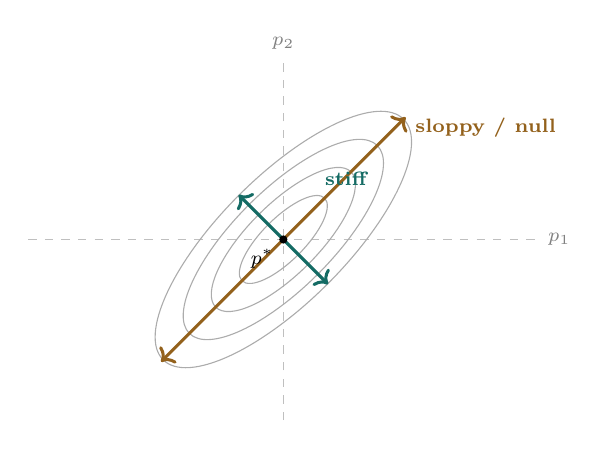
\begin{tikzpicture}[scale=1.35]
  \draw[dashed, gray!50] (-2.4,0) -- (2.4,0) node[right, gray] {\scriptsize $p_1$};
  \draw[dashed, gray!50] (0,-1.7) -- (0,1.7) node[above, gray] {\scriptsize $p_2$};
  \foreach \a/\b in {0.55/0.2, 0.9/0.33, 1.25/0.46, 1.6/0.59} {
    \draw[gray!65, thin, rotate around={45:(0,0)}] (0,0) ellipse ({\a} and {\b});
  }
  \draw[<->, thick, sloppycol, line width=1.1pt] (-1.15,-1.15) -- (1.15,1.15);
  \node[sloppycol, right] at (1.15,1.05) {\scriptsize\textbf{sloppy / null}};
  \draw[<->, thick, stiffcol, line width=1.1pt] (-0.42,0.42) -- (0.42,-0.42);
  \node[stiffcol, above right] at (0.30,0.42) {\scriptsize\textbf{stiff}};
  \fill (0,0) circle (1.1pt);
  \node[below left] at (0,0) {\scriptsize $p^*$};
\end{tikzpicture}
\caption{Contours of the objective near a fit $p^*$. The \slop{amber} and
\stiff{teal} axes are the valley's own directions, not the raw $p_1,p_2$ axes
(grey, dashed). A penalty built directly from $p_1$ and $p_2$ individually
cannot avoid mixing both.}
\label{fig:valley}
\end{figure}

The rest of this note builds a penalty aligned with the amber axis and
nothing else. First we need a way to \emph{find} that axis numerically --
that is what the Fisher Information Matrix (FIM) gives us.

\section{Setup: the local quadratic model}

Expand the objective around a reference point $p^*$ (typically your best fit
so far). To second order, with the first-order term vanishing at a fit,
\begin{equation}
  \mathrm{obj}(p) \;\approx\; \mathrm{obj}(p^*) \;+\; \tfrac{1}{2}\,(p-p^*)^\top H\,(p-p^*),
\end{equation}
where $H$ is the Gauss--Newton Hessian -- the same quantity
\file{fim\_l2\_constraintL2.R} already computes as \code{o\_best\$hessian},
i.e.\ $H = S^\top W S$ with $S$ the sensitivities and $W$ the inverse-variance
weights. This \emph{is} the Fisher Information Matrix.

\subsection*{Why expand around a point at all?}

This step is not a formality separate from ``just take the Hessian'' -- it is what makes
$H$ well defined in the first place. dMod's objective is built from ODE solutions and is
generally nonlinear in $p$; there is no single, global ``Hessian of the model'' the way
there would be for an actually-quadratic objective. What exists is $H = \nabla^2
\mathrm{obj}(p^*)$, the curvature \emph{at one specific point} -- evaluate it somewhere
else and you get a different matrix, different eigenvectors, possibly a different flat
direction.

Two consequences follow directly from this:
\begin{itemize}
  \item $p^*$ is not just where $H$ happens to live -- it is also the point the penalty
  in Section~4 is centered on, $R(p) = \lambda(p-p^*)^\top P(p-p^*)$. The penalty acts on
  the \emph{displacement} $p-p^*$, and $p^*$ is the only point that displacement can
  meaningfully be measured from, since it is exactly where the curvature was measured.
  \item Everything built from $H$ -- the stiff/sloppy split, $V_{\mathrm{null}}$, the
  projector $P$ -- is therefore a \emph{local} description, accurate only near $p^*$
  (cf.\ ``Local, not global'' in Section~8). In the worked example below, the valley
  happens to be exactly straight everywhere, because the toy model depends on $u+v$
  globally and not just locally, which is why $H$ there is exact rather than a local
  approximation; for a generic nonlinear model this need not hold, and
  $V_{\mathrm{null}}$ found at $p^*$ should be treated as trustworthy only in a
  neighborhood of $p^*$.
\end{itemize}

Diagonalize it (\code{eig <- eigen(H, symmetric = TRUE)}):
\begin{equation}
  H \;=\; V\,\mathrm{diag}(s_1,\ldots,s_n)\,V^\top .
\end{equation}
$V$ is orthogonal -- its columns $v_1,\ldots,v_n$ are the curvature's own
axes, each perpendicular to every other. $s_i$ is how sharply the objective
curves along $v_i$: large $s_i$ means that direction is pinned down tightly
by the data (stiff); $s_i$ near zero means the data barely constrains it at
all (sloppy) -- moving along $v_i$ changes the objective almost not at all,
exactly what a structural non-identifiability looks like numerically.

\section{Splitting the space}

Sort the eigenvalues by size and threshold them -- you already do exactly
this:
\begin{equation}
  \texttt{is\_zero}_i \;=\; \mathbb{1}\big[\,|s_i| < 10^{-6}\cdot\max_j |s_j|\,\big].
\end{equation}
This splits the eigenbasis into two groups of columns:
\begin{itemize}
  \item $V_{\mathrm{stiff}}$ -- eigenvectors with non-negligible curvature: directions the data actually pins down.
  \item $V_{\mathrm{null}}$ -- eigenvectors with (numerically) zero curvature: directions the data says nothing about, i.e.\ the non-identifiable group, expressed in its own natural coordinates rather than yours.
\end{itemize}
$V_{\mathrm{null}}$ is a set of \emph{directions} in parameter space,
generally a mix of several raw parameters (the amber axis in
Figure~\ref{fig:valley}), \emph{not} a subset of parameter names the way
\code{mu} in \code{constraintL2(mu, sigma)} is.

\section{The null-space penalty}

Build the matrix that projects any vector onto $V_{\mathrm{null}}$'s span:
\begin{equation}
  P \;=\; V_{\mathrm{null}}\,V_{\mathrm{null}}^\top .
\end{equation}
Because the columns of $V_{\mathrm{null}}$ are orthonormal, $P$ is symmetric
and \emph{idempotent}, $PP = P$ (projecting twice does nothing a single
projection didn't already do). Penalize only the component of $p$ that lands
inside that projection:
\begin{equation}
  R(p) \;=\; \lambda\,(p-p^*)^\top P\,(p-p^*) \;=\; \lambda\,\big\lVert V_{\mathrm{null}}^\top (p-p^*) \big\rVert^2 .
\end{equation}
The right-hand form is the more intuitive one: $z = V_{\mathrm{null}}^\top
(p-p^*)$ is just $p-p^*$ re-expressed in the sloppy eigenbasis, and $R =
\lambda\lVert z\rVert^2$ is an ordinary, isotropic L2 penalty -- but applied
to $z$, not to $p$. It is the same trick as regularizing ``only some
parameters,'' except the coordinates being regularized are a
rotated/projected combination discovered from the FIM, not a subset of names
picked by hand.

\subsection*{More than one null direction}

The worked example below has a single null eigenvalue, so $V_{\mathrm{null}}$
is one column, $v_1$. In general $m>1$ eigenvalues can come out
(numerically) zero at once, and the construction above does not change --
$V_{\mathrm{null}}$ just gets more columns:
\begin{equation}
  V_{\mathrm{null}} \;=\; \big[\,v_1 \mid v_2 \mid \cdots \mid v_m\,\big]
  \;=\;
  \begin{pmatrix}
    v_{1,1} & v_{2,1} & \cdots & v_{m,1}\\
    v_{1,2} & v_{2,2} & \cdots & v_{m,2}\\
    \vdots  & \vdots  &        & \vdots \\
    v_{1,n} & v_{2,n} & \cdots & v_{m,n}
  \end{pmatrix},
\end{equation}
an $n\times m$ \emph{matrix} -- $n$ rows, one per parameter, and $m$ columns,
one per null direction, placed \emph{side by side}. This is not the same as
concatenating the $v_i$ end to end into one length-$nm$ vector: that would
throw away exactly the structure $P=V_{\mathrm{null}}V_{\mathrm{null}}^\top$
needs to come back out as an $n\times n$ matrix, $(n\times m)\cdot(m\times
n)=n\times n$, the same shape $H$ has regardless of $m$. Equivalently, this
matrix product is the sum of the $m$ individual rank-1 projectors,
\begin{equation}
  P \;=\; V_{\mathrm{null}}V_{\mathrm{null}}^\top \;=\; \sum_{i=1}^m v_iv_i^\top,
\end{equation}
and every property established above -- symmetric, idempotent ($P^2=P$,
because $V_{\mathrm{null}}^\top V_{\mathrm{null}}=I_m$ regardless of $m$),
rank exactly $m$ -- carries over unchanged; nothing in that argument used
$m=1$.

The two expressions in the equation above are not merely analogous --
``compute each single-vector projector $v_iv_i^\top$ and add them up'' is
exactly what the matrix product $V_{\mathrm{null}}V_{\mathrm{null}}^\top$
does, entry for entry. Multiplying an $n\times m$ matrix by its transpose
sums over the shared index, which here is the $m$ columns:
\begin{equation}
  V_{\mathrm{null}}V_{\mathrm{null}}^\top
  \;=\;
  \begin{pmatrix}\mid&&\mid\\ v_1&\cdots&v_m\\ \mid&&\mid\end{pmatrix}
  \begin{pmatrix}-\,v_1^\top\,-\\ \vdots\\ -\,v_m^\top\,-\end{pmatrix}
  \;=\;
  v_1v_1^\top + v_2v_2^\top + \cdots + v_mv_m^\top,
\end{equation}
the standard ``matrix times its own transpose = sum of outer products of its
columns'' identity, nothing specific to this construction. So there is no
choice to make between ``add the single-vector projectors'' and ``form
$V_{\mathrm{null}}V_{\mathrm{null}}^\top$'' -- they are the same arithmetic,
one written as $m$ separate $n\times n$ sums, the other as one matrix
product that performs those sums internally.

\paragraph{A three-parameter illustration.} Extend the model to $u,v,w$
entering the data only through $u+v+w$ (e.g.\ a product of three rates).
Then $H=c\begin{pmatrix}1&1&1\\1&1&1\\1&1&1\end{pmatrix}$: one stiff
eigenvalue $3c$ along $(1,1,1)/\sqrt3$, and a \emph{two}-dimensional null
eigenspace -- everything orthogonal to $(1,1,1)$. Picking any orthonormal
basis of that plane, e.g.\ $v_2=(1,-1,0)/\sqrt2,\ v_3=(1,1,-2)/\sqrt6$,
\begin{equation}
  P \;=\; v_2v_2^\top+v_3v_3^\top \;=\; \begin{pmatrix}2/3&-1/3&-1/3\\-1/3&2/3&-1/3\\-1/3&-1/3&2/3\end{pmatrix}
  \;=\; I-\tfrac13 J,
\end{equation}
where $J$ is the all-ones matrix -- the familiar ``mean-centering'' projector
from statistics. This was computed by adding the two individual projectors
directly, and by the identity above it is the same matrix
$V_{\mathrm{null}}V_{\mathrm{null}}^\top$ would give for
$V_{\mathrm{null}}=[v_2\mid v_3]$ -- either route, same $P$. Same penalty
formula as before, $R=\lambda\,\delta^\top P\,\delta$, now pulling any drift
within the two-dimensional gauge back to $p^*$ while leaving $u+v+w$
untouched.

A repeated eigenvalue also means \code{eigen()}'s particular choice of
$v_2,v_3$ \emph{within} that plane is arbitrary -- a different orthonormal
basis of the same plane prints different numbers. $P$ does not care: for any
orthogonal $Q$ ($Q^\top Q=I$), replacing $V_{\mathrm{null}}\to
V_{\mathrm{null}}Q$ gives $P'=V_{\mathrm{null}}QQ^\top
V_{\mathrm{null}}^\top=V_{\mathrm{null}}V_{\mathrm{null}}^\top=P$ --
unchanged. $P$ depends only on the null \emph{subspace}, never on which
orthonormal basis of it happened to come out of the eigensolver. In code,
none of this needs special-casing either: \code{V\_null <-
eig\$vectors[, is\_zero, drop = FALSE]} (``From formula to code'' below)
already places columns side by side whenever \code{is\_zero} flags more than
one direction, and \code{P <- V\_null \%*\% t(V\_null)} is the same matrix
product whether $m=1$ or $m=2$.

\subsection*{From projector to penalty, directly}

There is a second, more direct route to the same formula, worth seeing
because it starts from something completely familiar: an ordinary ridge
penalty, $R_{\mathrm{naive}}(p)=\lambda\lVert\delta\rVert^2=\lambda\,\delta^\top
I\,\delta$ ($I$ the identity), penalizes \emph{every} component of
$\delta=p-p^*$ equally -- including the identified direction, exactly what
Section~4.3 shows must not happen. Now swap out ``the whole displacement''
for ``only its null-space component'': $P\delta$ keeps just $\delta$'s piece
along $V_{\mathrm{null}}$ and discards everything along $V_{\mathrm{stiff}}$
-- that is what a projector does by definition -- so penalize $\lVert
P\delta\rVert^2$ instead of $\lVert\delta\rVert^2$:
\begin{equation}
  R(p) \;=\; \lambda\,\lVert P\delta\rVert^2.
\end{equation}
This is still just an ordinary L2 penalty, only applied to $P\delta$ rather
than to $\delta$ itself. Expanding the square, $\lVert P\delta\rVert^2 =
\delta^\top P^\top P\,\delta$, and because $P$ is symmetric and idempotent
(established two paragraphs up), $P^\top P = P^2 = P$, so
\begin{equation}
  R(p) \;=\; \lambda\,\delta^\top P\,\delta,
\end{equation}
the same formula as above, with no $V_{\mathrm{null}}$ coordinate change
needed once $P$ itself is in hand. In short: take an ordinary ridge penalty
and swap $I$ for $P$; idempotency does the rest, collapsing ``penalize the
projected vector'' and ``penalize with the projector as the quadratic form''
into the same expression.

\paragraph{In the worked example.} $P=\begin{pmatrix}0.5&-0.5\\-0.5&0.5\end{pmatrix}$
(Section~6), so
\begin{equation}
  R(u,v) \;=\; \lambda\begin{pmatrix}\delta_u&\delta_v\end{pmatrix}
  \begin{pmatrix}0.5&-0.5\\-0.5&0.5\end{pmatrix}
  \begin{pmatrix}\delta_u\\\delta_v\end{pmatrix}
  \;=\; \lambda\big(0.5\delta_u^2 - \delta_u\delta_v + 0.5\delta_v^2\big)
  \;=\; \tfrac12\lambda(\delta_u-\delta_v)^2,
\end{equation}
exactly the penalty derived in Section~6 -- reached here directly from $P$,
without first passing through the $z=V_{\mathrm{null}}^\top\delta$ coordinate
change below.

\subsection*{From the eigenbasis back to the original parameters}

Two different spaces are involved here, and it is worth being explicit about
how one maps into the other, so that $R(p)$ does not look like a change of
variables smuggled into the objective.

Let $\delta = p-p^*$, an $n$-vector in the \emph{original} parameter space --
the same space the rest of the objective, its gradient, and its Hessian all
live in. Because $V = (V_{\mathrm{stiff}} \mid V_{\mathrm{null}})$ is a full
orthogonal basis of that same $\mathbb{R}^n$ (Section~2), $\delta$ splits
exactly, with nothing left over and nothing changed about which space it
lives in:
\begin{equation}
  \delta \;=\; VV^\top\delta \;=\;
  \underbrace{V_{\mathrm{stiff}}V_{\mathrm{stiff}}^\top\delta}_{\delta_{\mathrm{stiff}}}
  \;+\;
  \underbrace{V_{\mathrm{null}}V_{\mathrm{null}}^\top\delta}_{\delta_{\mathrm{null}}}.
\end{equation}
$\delta_{\mathrm{stiff}}$ and $\delta_{\mathrm{null}}$ are themselves still
$n$-vectors in the original space -- resolving $\delta$ along the $v_i$ axes
and adding the pieces back up, exactly as resolving a 2D vector into its
$x$- and $y$-components and summing them returns the original vector.

The reduced, $m$-dimensional eigenspace ($m$ = number of null directions)
only enters as the \emph{coordinates} of $\delta_{\mathrm{null}}$ within
that subspace,
\begin{equation}
  z \;=\; V_{\mathrm{null}}^\top\delta \;\in\;\mathbb{R}^m
  \qquad\text{(``analysis'': how far along each null direction).}
\end{equation}
This genuinely is a smaller, different space -- $z$ has no notion of
``which raw parameter'' left, only ``how far along null-direction 1, 2,
\ldots''. It is precisely in this space that an isotropic penalty $R =
\lambda\lVert z\rVert^2$ is the unbiased choice: every direction spanned by
$V_{\mathrm{null}}$ is, by construction, equally unconstrained by the data,
so there is no reason to weight one over another once you are in the basis
where ``isotropic'' means exactly ``no preference among directions the data
is silent on.''

Substituting $z$ back undoes the detour (``synthesis''):
\begin{equation}
  R \;=\; \lambda z^\top z
  \;=\; \lambda(V_{\mathrm{null}}^\top\delta)^\top(V_{\mathrm{null}}^\top\delta)
  \;=\; \lambda\,\delta^\top\underbrace{V_{\mathrm{null}}V_{\mathrm{null}}^\top}_{P}\delta,
\end{equation}
so $P\delta = V_{\mathrm{null}}z$ is nothing but $\delta_{\mathrm{null}}$
again, re-expanded from its $m$ coordinates back into the original
$n$-dimensional space. $P$ is therefore analysis-then-synthesis fused into a
single $n\times n$ matrix: project onto the null coordinates, then
immediately re-embed. The $m$-dimensional detour is real but never has to be
materialized at evaluation time -- $R(p) = \lambda\delta^\top P\delta$, and
likewise $\nabla R = 2\lambda P\delta$ and $\nabla^2 R = 2\lambda P$ below,
are closed formulas that take $p\in\mathbb{R}^n$ in and return an
$n$-vector / $n\times n$-matrix out, indexed by the same raw parameter names
as the rest of the objective -- exactly what \code{"+.fn"} needs to add
\code{prior\_group}'s gradient/Hessian to \code{obj}'s elementwise.

Note $P$ is only positive \emph{semi}-definite, rank $m<n$: it vanishes
exactly on $V_{\mathrm{stiff}}$'s span. That degeneracy is the design goal,
not a defect -- $R$ is a genuine function on all of $\mathbb{R}^n$, evaluated
on the full $p$, that is deliberately blind to the stiff subspace, which is
what makes the ``untouched identified combination'' property below hold
exactly rather than approximately.

\subsection*{Value, gradient, Hessian}

Because $R$ is exactly quadratic, all three are closed-form and exact -- no
chain rule, no \code{deriv2} needed:
\begin{equation}
  \nabla R \;=\; 2\lambda P\,(p-p^*), \qquad \nabla^2 R \;=\; 2\lambda P \quad\text{(constant, independent of $p$).}
\end{equation}

\subsection*{Combining with the data objective}

$R$ is not the objective you actually minimize -- it is one summand of it.
Write $L_{\mathrm{data}}$ for whatever \code{obj} you started with (a
\code{normL2} on its own, or already a sum with other
\code{constraintL2}/\code{priorL2} terms). The fitted objective is
\begin{equation}
  L_{\mathrm{tot}}(p) \;=\; L_{\mathrm{data}}(p) \;+\; R(p),
\end{equation}
and because \code{"+.objlist"} (\file{R/objClass.R}, around line 875) adds
the \code{value}/\code{gradient}/\code{hessian} slots of two \code{objlist}s
elementwise, matched by parameter name (union-and-zero-pad if the name sets
differ, intersect-and-add if one is a subset of the other), this holds
termwise and exactly, for \emph{any} $L_{\mathrm{data}}$, not just a
quadratic one:
\begin{align}
  \nabla L_{\mathrm{tot}}(p) &\;=\; \nabla L_{\mathrm{data}}(p) \;+\; 2\lambda P\,(p-p^*), \\
  \nabla^2 L_{\mathrm{tot}}(p) &\;=\; \nabla^2 L_{\mathrm{data}}(p) \;+\; 2\lambda P.
\end{align}
Two things are worth noting about this sum:
\begin{itemize}
  \item $L_{\mathrm{data}}$ need not be quadratic or even close to it -- $R$'s
  contribution is exact regardless, since $R$ was built to be exactly
  quadratic on its own (Section~4.1). Only $L_{\mathrm{data}}$'s own
  value/gradient/Hessian have to come from the usual \code{deriv}/\code{deriv2}
  machinery; $R$ never needs it.
  \item $\nabla^2 R = 2\lambda P$ is \emph{constant} in $p$, so its contribution
  to $\nabla^2 L_{\mathrm{tot}}$ is the same fixed matrix at every iterate --
  only $\delta = p-p^*$ in the gradient term, and $\nabla^2 L_{\mathrm{data}}$
  itself, change as the optimizer moves.
\end{itemize}
In code this is exactly \code{obj\_group <- obj + prior\_group} from
Section~6: \code{obj} supplies $L_{\mathrm{data}}$'s \code{objlist},
\code{prior\_group} supplies $R$'s, and \code{"+.fn"}/\code{"+.objlist"}
perform the sum above automatically, with no special-casing needed for the
fact that one summand came from an ODE fit and the other from a fixed
projector matrix.

\subsection*{Why the identified combination is untouched}

Take any displacement $\delta$ that lies purely in the stiff subspace,
$\delta = V_{\mathrm{stiff}}\,c$ for some coefficients $c$. Since $V$'s
columns are mutually orthogonal by construction, $V_{\mathrm{null}}^\top
V_{\mathrm{stiff}} = 0$, so
\begin{equation}
  P\delta \;=\; V_{\mathrm{null}}\big(V_{\mathrm{null}}^\top V_{\mathrm{stiff}}\big)c \;=\; 0
  \qquad\text{exactly, not approximately -- for any $c$.}
\end{equation}
$R$ and its gradient are \emph{identically} zero for any move confined to the
identified directions. This is the property a per-parameter
\code{constraintL2} prior cannot offer: unless a sloppy eigenvector happens
to line up with one raw parameter axis, no choice of diagonal $\sigma_i$ can
null out a direction exactly -- it can only make the leakage smaller.

\section{Worked example}

Take the multiplicative symmetry discussed earlier: a model where only the
product $k_1 k_2$ is identifiable, not $k_1$ and $k_2$ separately. Working in
dMod's usual log-parametrization, $u = \log k_1$, $v = \log k_2$, the data
only ever sees $u+v$. Near the fit, with data-curvature constant $c$ along
$u+v$, the objective's curvature is
\begin{equation}
  H \;=\; c\begin{pmatrix}1&1\\1&1\end{pmatrix}, \qquad c = 4.
\end{equation}
This $H$ is exactly singular -- not just small in one direction, genuinely
zero -- which makes the eigendecomposition easy to do by hand.

\subsection*{Where this $H$ comes from}

It is still the same Gauss--Newton Hessian $H=S^\top WS$ from Section~2, just
specialized to a toy model simple enough to write down by hand instead of
computing numerically. The model prediction depends on $u,v$ only through the
sum $u+v$ (since $k_1k_2=e^{u+v}$), so for every data point $k$ the chain rule
gives
\begin{equation}
  \frac{\partial y_k}{\partial u} \;=\; \frac{\partial y_k}{\partial(u+v)}\cdot 1
  \;=\; \frac{\partial y_k}{\partial v},
\end{equation}
i.e.\ the sensitivities w.r.t.\ $u$ and $v$ are identical, point for point --
there is only one sensitivity direction here, not two independent ones.
Substituting into $H=S^\top WS$,
\begin{equation}
  H_{uu} = \sum_k\Big(\tfrac{\partial y_k}{\partial u}\Big)^{\!2} w_k, \quad
  H_{uv} = \sum_k \tfrac{\partial y_k}{\partial u}\tfrac{\partial y_k}{\partial v}\,w_k, \quad
  H_{vv} = \sum_k\Big(\tfrac{\partial y_k}{\partial v}\Big)^{\!2} w_k
\end{equation}
all three sums are the same sum, because the two derivatives being summed are
equal everywhere. Calling that common value $c$ reproduces exactly the matrix
above -- a rank-1 $H$ whose only nonzero eigenvalue lies along $(1,1)/\sqrt2$,
the identified direction $u+v$, and whose eigenvalue along $(1,-1)/\sqrt2$ is
exactly zero. $c=4$ is not derived from a specific dataset here; it is the
aggregate curvature $\sum_k(\partial y_k/\partial(u+v))^2w_k$ along $u+v$,
fixed at a round number so the eigendecomposition below comes out clean. In
the actual code (\file{fim\_l2\_constraintL2.R}), this is exactly where
\code{o\_best\$hessian} would instead be a real, numerically computed
Gauss--Newton Hessian built from the model's actual $S$ and $W$.

\subsection*{Why this toy model can be differentiated by hand at all}

The reason the sensitivities above can be written down as a clean chain-rule
step rather than pulled out of a solver is that this particular model is
linear and solvable in closed form. Take a plain one-step handoff,
\begin{equation}
  \dot A \;=\; -kqA, \qquad \dot B \;=\; kqA, \qquad A(0)=A_0,\ B(0)=0,
\end{equation}
with $K=kq=e^{u+v}$ ($u=\log k,\ v=\log q$) -- $B$ has no decay of its own,
it only ever receives what $A$ loses, so $A(t)+B(t)=A_0$ for all $t$ (mass
conservation). Solving,
\begin{equation}
  A(t) = A_0e^{-Kt}, \qquad B(t) = A_0\big(1-e^{-Kt}\big).
\end{equation}
Both are functions of $u,v$ only through $K$, and $\partial K/\partial u =
\partial K/\partial v = K$ (since $K=e^{u+v}$ -- the same structural fact
driving the whole null-space argument), so differentiating the closed forms
directly gives
\begin{equation}
  \frac{\partial A}{\partial u} \;=\; \frac{\partial A}{\partial K}\cdot K
  \;=\; \big({-}tA_0e^{-Kt}\big)K \;=\; \frac{\partial A}{\partial v},
  \qquad
  \frac{\partial B}{\partial u} \;=\; \big(tA_0e^{-Kt}\big)K \;=\; \frac{\partial B}{\partial v},
\end{equation}
by hand, no solver involved -- and note $\partial B/\partial K = -\partial
A/\partial K$ exactly, a direct consequence of $A+B\equiv A_0$: whatever $A$
loses in sensitivity, $B$ gains, at every $t$. This is the same object dMod
computes numerically for a general (non-solvable) model: the sensitivity
ODEs for $S_A=\partial A/\partial p,\ S_B=\partial B/\partial p$ are obtained
by differentiating $\dot A=-KA,\ \dot B=KA$ themselves w.r.t.\ $p$ and
swapping the order of $\partial_t,\partial_p$,
\begin{equation}
  \dot S_A \;=\; -\frac{\partial K}{\partial p}A \;-\; K\,S_A,
  \qquad
  \dot S_B \;=\; \frac{\partial K}{\partial p}A \;+\; K\,S_A \;=\; -\dot S_A,
\end{equation}
a pair of linear ODEs that -- because $A(t),B(t)$ happen to have closed forms
here -- can also be solved by hand, reproducing exactly $\partial A/\partial
K\cdot\partial K/\partial p$ and its negative above (and confirming
$S_A+S_B\equiv 0$, the sensitivity-level statement of mass conservation).
``Solve the ODE, then differentiate the solution'' and ``differentiate the
ODE, then solve the resulting sensitivity ODE'' are the same computation; the
toy example only gets to skip the numerical integrator because it is linear
enough to do both steps in closed form. \code{Xs(..., deriv = TRUE)}
(\file{R/prediction.R}) takes the second route unconditionally -- it
symbolically differentiates the ODE right-hand side, stacks the resulting
variational equations onto the state ODE, and integrates state and
sensitivities together in one solver call -- which is the only route
available once the model has no closed-form solution, i.e.\ essentially
every real dMod model.

\subsection*{The Hessian, entry by entry}

Collecting the four sensitivities from above, $\partial A_t/\partial u =
\partial A_t/\partial v = -tKA(t)$ and $\partial B_t/\partial u = \partial
B_t/\partial v = tKA(t)$, and writing $w_A(t), w_B(t)$ for the inverse-variance
weight of an $A$- and $B$-observation at time $t$, each entry of $H=S^\top WS$
is its own sum over the data, observable by observable, with nothing
simplified or cancelled yet:
\begin{equation}
  \resizebox{\textwidth}{!}{$
  H \;=\;
  \begin{pmatrix}
    \displaystyle\sum_t\Big[\big({-}tKA(t)\big)^2 w_A(t) \,+\, \big(tKA(t)\big)^2 w_B(t)\Big]
    &
    \displaystyle\sum_t\Big[\big({-}tKA(t)\big)\big({-}tKA(t)\big) w_A(t) \,+\, \big(tKA(t)\big)\big(tKA(t)\big) w_B(t)\Big]
    \\[16pt]
    \displaystyle\sum_t\Big[\big({-}tKA(t)\big)\big({-}tKA(t)\big) w_A(t) \,+\, \big(tKA(t)\big)\big(tKA(t)\big) w_B(t)\Big]
    &
    \displaystyle\sum_t\Big[\big({-}tKA(t)\big)^2 w_A(t) \,+\, \big(tKA(t)\big)^2 w_B(t)\Big]
  \end{pmatrix}
  $}
\end{equation}
Top-left is $H_{uu}=\sum_t(\partial A_t/\partial u)^2w_A + (\partial
B_t/\partial u)^2w_B$; top-right is $H_{uv}=\sum_t(\partial A_t/\partial
u)(\partial A_t/\partial v)w_A + (\partial B_t/\partial u)(\partial
B_t/\partial v)w_B$; bottom-left is the same sum as top-right by symmetry
($H_{vu}=H_{uv}$); bottom-right is $H_{vv}$, built the same way as $H_{uu}$
but with $\partial/\partial v$ in place of $\partial/\partial u$ -- which,
substituted in, is the identical expression, since $\partial A_t/\partial u
=\partial A_t/\partial v$ and $\partial B_t/\partial u=\partial B_t/\partial
v$ pointwise. All four entries are therefore, term by term,
$({-}x)^2=x\cdot x=({-}x)({-}x)=x^2$ for $x=tKA(t)$ -- algebraically forced to
be the same expression before any sum is even evaluated. Calling that common
sum $c$,
\begin{equation}
  c \;=\; \sum_t \big(tKA(t)\big)^2\big[w_A(t)+w_B(t)\big],
\end{equation}
reproduces $H=c\big(\begin{smallmatrix}1&1\\1&1\end{smallmatrix}\big)$ exactly
-- now with $c$ tied to a concrete formula in $t$, $K$, $A(t)$ and the two
observables' weights, rather than the placeholder value $c=4$ used earlier for
the by-hand eigendecomposition.

\subsection*{What if only $A$ is observed?}

Nothing about the null-space structure changes -- $B$'s term simply drops out
of the sum. $A(t)=A_0e^{-Kt}$ is a function of $u,v$ only through $K$, exactly
as before, so $\partial A_t/\partial u=\partial A_t/\partial v=-tKA(t)$ still
holds pointwise, and every entry of $H$ collapses to the same single sum as
above with the $w_B(t)$ term removed:
\begin{equation}
  H_{uu}=H_{uv}=H_{vv} \;=\; \sum_t\big(tKA(t)\big)^2w_A(t) \;=:\; c_A,
  \qquad H \;=\; c_A\begin{pmatrix}1&1\\1&1\end{pmatrix}.
\end{equation}
Still exactly rank-1, still $V_{\mathrm{null}}=(1,-1)/\sqrt2$, still the same
projector $P$ and penalty $R(u,v)=\tfrac12\lambda(\delta_u-\delta_v)^2$ from
Section~4 -- only $c$ shrinks, since dropping $B$'s data removes curvature
along $u+v$ but not along any new direction (it was never contributing any).

This has to be true, not just happen to be true here: every state in this
model, not only $A$ and $B$, is a function of $t$ and $K$ alone -- the
symmetry $k\to ck,\ q\to q/c$ leaves $K$, and hence the entire trajectory,
invariant. That is a property of the state-space equations themselves, fixed
before any observation function is chosen. So no choice of what to
observe -- $A$ alone, $B$ alone, or both -- can ever see $u-v$; only observing
something that depends on $k,q$ through a genuinely different combination
than $K$ could. This is exactly why \code{symmetryDetection()}
(\file{R/symmetryDetection.R}, referenced in Section~8) certifies a
\emph{structural} symmetry on the state-space model directly, independent of
\code{Y()} -- it holds for any observable you could construct from the
states, which is precisely what the calculation above just confirmed by hand.

\begin{table}[h]
\centering
\begin{tabular}{@{}lll@{}}
\toprule
eigenvalue $s$ & eigenvector $v$ & reading \\
\midrule
$8$ & $(1,\,1)/\sqrt{2}$ & \stiff{stiff} -- the identified direction, $u+v$ \\
$0$ & $(1,\,-1)/\sqrt{2}$ & \slop{sloppy} -- the null direction, $u-v$ \\
\bottomrule
\end{tabular}
\caption{Eigendecomposition of $H$.}
\end{table}

So $V_{\mathrm{null}} = (1,-1)/\sqrt{2}$, and the projector is
\begin{equation}
  P \;=\; V_{\mathrm{null}}V_{\mathrm{null}}^\top \;=\; \begin{pmatrix}0.5 & -0.5\\ -0.5 & 0.5\end{pmatrix}.
\end{equation}
Writing $\delta = (\delta_u,\delta_v) = (u-u^*,\,v-v^*)$, the penalty reduces
to a single term:
\begin{equation}
  R(u,v) \;=\; \tfrac{1}{2}\lambda\,(\delta_u - \delta_v)^2,
\end{equation}
which depends \emph{only} on the gap $\delta_u - \delta_v$ -- i.e.\ only on
how far the current gauge has drifted from the reference gauge -- never on
$\delta_u+\delta_v$, the quantity the data actually fits.

\subsection*{The combined objective, concretely}

Writing $L_{\mathrm{data}}(u,v)$ for whatever the fit's own objective is
(some nonlinear function of $u,v$ near $p^*$, of which $H$ above is just the
local curvature), the general combination formula from Section~4.2
instantiates to
\begin{equation}
  L_{\mathrm{tot}}(u,v) \;=\; L_{\mathrm{data}}(u,v) \;+\; \tfrac{1}{2}\lambda\,(\delta_u-\delta_v)^2,
\end{equation}
\begin{equation}
  \nabla L_{\mathrm{tot}} \;=\; \nabla L_{\mathrm{data}} \;+\;
  \begin{pmatrix}\lambda(\delta_u-\delta_v)\\[2pt] -\lambda(\delta_u-\delta_v)\end{pmatrix},
  \qquad
  \nabla^2 L_{\mathrm{tot}} \;=\; \nabla^2 L_{\mathrm{data}} \;+\; \lambda\begin{pmatrix}1&-1\\-1&1\end{pmatrix}.
\end{equation}
This is a direct numerical check of the ``untouched'' claim from
Section~4.3: move along the stiff/data direction, $\delta_u=\delta_v$ (any
displacement of the form $c\cdot(1,1)$), and the penalty's contribution to
the gradient is $\lambda(\delta_u-\delta_v)=0$ exactly, and to the Hessian,
applied to that same direction, $\lambda\left(\begin{smallmatrix}1&-1\\-1&1\end{smallmatrix}\right)\left(\begin{smallmatrix}1\\1\end{smallmatrix}\right) = \left(\begin{smallmatrix}0\\0\end{smallmatrix}\right)$
-- the penalty is invisible along $u+v$ and only bends $L_{\mathrm{tot}}$
along $u-v$, exactly the gauge direction it was built to constrain.

\subsection*{Two observables, one with a flipped sign}

Suppose the model has two observables $A,B$ instead of one, and (as in
\file{scripts/example\_toy\_fit.R}, where the $A\to B$ rate is
\code{k1*q1*A} so only $K=k_1q_1=e^{u+v}$ ever enters the ODE) both depend on
$u,v$ only through that same combination -- but with opposite sign,
\begin{equation}
  y_{A,k} \;=\; h_A\big({-}(u+v)\big), \qquad y_{B,k} \;=\; h_B(u+v).
\end{equation}
It is tempting to expect the minus sign to change the null-space calculation.
It does not. By the chain rule,
\begin{equation}
  \frac{\partial y_{A,k}}{\partial u} \;=\; -h_A'\big({-}(u{+}v)\big) \;=\;
  \frac{\partial y_{A,k}}{\partial v},
  \qquad
  \frac{\partial y_{B,k}}{\partial u} \;=\; h_B'(u{+}v) \;=\; \frac{\partial y_{B,k}}{\partial v},
\end{equation}
so $\partial y/\partial u=\partial y/\partial v$ still holds for \emph{every}
residual, from either observable -- the sign of the coefficient in front of
$(u+v)$ never breaks that equality, only using a genuinely different
combination (e.g.\ $u-v$) would. Summing $H=S^\top WS$ over both observables'
residuals together,
\begin{equation}
  H_{uu} = \sum_k\Big(\tfrac{\partial y_k}{\partial u}\Big)^{\!2}w_k, \quad
  H_{uv} = \sum_k\tfrac{\partial y_k}{\partial u}\tfrac{\partial y_k}{\partial v}w_k, \quad
  H_{vv} = \sum_k\Big(\tfrac{\partial y_k}{\partial v}\Big)^{\!2}w_k,
\end{equation}
A's residuals contribute $(-h_A')(-h_A')=(h_A')^2$ to $H_{uv}$ -- positive,
identical to their own contribution to $H_{uu}$ and $H_{vv}$ -- because the
minus sign appears \emph{twice} (once from each partial derivative) and
cancels in the product. Writing $c_A=\sum_{k\in A}(h_A')^2w_k$ and
$c_B=\sum_{k\in B}(h_B')^2w_k$, the two observables' curvatures simply add:
\begin{equation}
  H \;=\; (c_A+c_B)\begin{pmatrix}1&1\\1&1\end{pmatrix}.
\end{equation}
The sign changes nothing about $H$'s shape -- still rank-1, still
$V_{\mathrm{null}}=(1,-1)/\sqrt2$ -- it only folds into $c$, now a sum of both
observables' contributions instead of one. Intuitively: the sign flip matters
for the \emph{gradient} (it flips which way $A$'s residual pulls the fit) but
not the Hessian, which is quadratic in the sensitivities and so blind to a
uniform sign flip applied to both partials at once. Adding observable $A$
supplies more data along the identified direction $u+v$; it supplies nothing
about $u-v$, so it does not touch the non-identifiability at all. That would
only happen if $A$ depended on a genuinely different combination, such as
$u-v$ itself.

\section{Naive vs.\ projector, side by side}

Compare the gradients of the two penalties directly. ``Naive'' is
\code{constraintL2(mu = c(u=u*, v=v*), sigma = c(}$\sigma,\sigma$\code{))},
i.e.\ $R_{\mathrm{naive}} = (\delta_u^2+\delta_v^2)/\sigma^2$. The number
that matters is $\partial R/\partial u + \partial R/\partial v$ -- the net
push along the stiff direction $(1,1)$, i.e.\ against the identified
combination:

\begin{table}[h]
\centering
\begin{tabular}{@{}lccl@{}}
\toprule
 & $\partial R/\partial u$ & $\partial R/\partial v$ & sum (pull on $u+v$) \\
\midrule
naive, diagonal & $2\delta_u/\sigma^2$ & $2\delta_v/\sigma^2$ &
  $2(\delta_u+\delta_v)/\sigma^2$ -- \textbf{nonzero} unless $\delta_u=-\delta_v$ \\
projector & $\lambda(\delta_u-\delta_v)$ & $-\lambda(\delta_u-\delta_v)$ &
  \stiff{$0$ -- always, for every $\delta$} \\
\bottomrule
\end{tabular}
\caption{Net pull on the identified combination $u+v$.}
\end{table}

The naive penalty's sum is zero only on the razor's edge where
$\delta_u=-\delta_v$ exactly -- everywhere else it quietly drags the fit's
best-supported quantity, $u+v$, toward $u^*+v^*$ too, competing with the data
even though the data already had an opinion there. The projector's sum is
zero identically -- it has no opinion about $u+v$ at all, by construction.

\begin{figure}[h]
\centering
\begin{minipage}{0.46\textwidth}
\centering
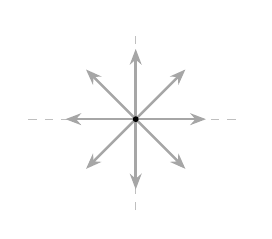
\begin{tikzpicture}[scale=1.05]
  \draw[dashed, gray!50] (-1.3,0) -- (1.3,0);
  \draw[dashed, gray!50] (0,-1.1) -- (0,1.1);
  \foreach \ang in {0,45,90,135,180,225,270,315} {
    \draw[-{Stealth[length=2mm]}, gray!70, line width=0.9pt]
      (0,0) -- (\ang:0.85);
  }
  \fill (0,0) circle (1pt);
\end{tikzpicture}

\footnotesize Naive: equal pull regardless of what the\\data already knows.
\end{minipage}
\hfill
\begin{minipage}{0.46\textwidth}
\centering
\begin{tikzpicture}[scale=1.05]
  \draw[dashed, gray!50] (-1.3,0) -- (1.3,0);
  \draw[dashed, gray!50] (0,-1.1) -- (0,1.1);
  \draw[<->, sloppycol, -{Stealth[length=2.2mm]}, line width=1.2pt] (-0.6,-0.6) -- (0.6,0.6);
  \node[stiffcol] at (0.68,-0.35) {\scriptsize $0$};
  \node[stiffcol] at (-0.68,0.35) {\scriptsize $0$};
  \fill (0,0) circle (1pt);
\end{tikzpicture}

\footnotesize Projector: pull confined to $V_{\mathrm{null}}$;\\the stiff direction reads exactly $0$.
\end{minipage}
\caption{Naive isotropic pull (left) vs.\ null-space projector pull (right).}
\end{figure}

\section{From formula to code}

\code{constraintL2()} cannot express this directly -- it only builds a
diagonal penalty in the raw parameter names (\file{R/objClass.R}, around line
433). $P$ is generally dense, so the penalty needs its own small
\code{objfn}, built the same way \code{constraintL2} is: return an
\code{objlist} with exact value, gradient and Hessian, and let \code{+} fold
it into the rest of the objective.

\begin{lstlisting}
# H, eig, s, is_zero, best already computed in fim_l2_constraintL2.R, Part 8
V_null <- eig$vectors[, is_zero, drop = FALSE]   # n x m, m = # non-identifiable directions
P      <- V_null %*% t(V_null)                   # n x n projector, symmetric, P %*% P == P

groupL2 <- function(P, p0, lambda = 0.1) {
  force(P); force(p0); force(lambda)
  function(..., fixed = NULL, deriv = TRUE, deriv2 = FALSE,
           conditions = NULL, env = NULL) {
    p     <- list(...)[[1]]
    delta <- p[names(p0)] - p0
    Pd    <- as.numeric(P %*% delta)

    value <- lambda * sum(delta * Pd)              # R(p) = lambda * delta' P delta
    grad  <- setNames(2 * lambda * Pd, names(p0))   # exact, no deriv2 needed
    hess  <- 2 * lambda * P
    dimnames(hess) <- list(names(p0), names(p0))

    out <- objlist(value = value, gradient = grad, hessian = hess)
    attr(out, "prior") <- value
    attr(out, "env")   <- env
    out
  }
}

prior_group <- groupL2(P, best, lambda = 0.1)
class(prior_group) <- c("objfn", "fn")
attr(prior_group, "parameters") <- names(best)

obj_group <- obj + prior_group   # "+.fn" sums value / gradient / hessian, as usual
\end{lstlisting}

If \code{best} sits behind a \code{trafo}/\code{P()} reparameterization,
apply this at the same (outer) parameter level $H$ was computed at -- the
same level \code{constraintL2} already operates on -- so no extra chain rule
is required.

\section{Practical notes}

\paragraph{Local, not global.} $H$ is a snapshot at $p^*$. If the true
symmetry is curved in your raw parameters (it usually is not, once you are
already in log-space -- multiplicative symmetries become straight lines
exactly like the worked example), $V_{\mathrm{null}}$ is only accurate near
$p^*$; re-evaluate $H$ if the fit moves far from where it was computed.

\paragraph{Relation to your \code{sigma\_fim} construction.} The existing
anisotropic recipe uses a \emph{soft}, reciprocal weight $w_i =
\texttt{strength}/(s_i+\texttt{eps\_reg})$ for every eigendirection, then
keeps only the diagonal of $V\,\mathrm{diag}(w)\,V^\top$ -- every direction
gets \emph{some} pull, and cross-parameter structure is discarded when
collapsing to a diagonal $\sigma$. The projector above is the same
construction pushed to its limit: a \emph{hard} 0/1 weight (\code{is\_zero})
instead of a soft reciprocal one, and the full dense $P$ kept intact instead
of flattened to a diagonal. The result is a strict either/or: a direction is
either fully exempt or fully regularized, and the ``how strongly'' knob
($\lambda$) is decoupled from ``which directions'' (the mask) -- whereas
today those two questions are answered by the same number,
\code{strength / (s\_i + eps\_reg)}.

\paragraph{If you know the symmetry analytically.} When
\code{symmetryDetection()} (\file{R/symmetryDetection.R}) can name the
symmetry generator in closed form, that is strictly better than any
numerical $V_{\mathrm{null}}$: reparametrize via \code{repar()} into
(identified combination, gauge coordinate) directly, and
\code{constraintL2()} the gauge coordinate alone. $z = V_{\mathrm{null}}^\top
(p-p^*)$ above is exactly a numerical stand-in for that gauge coordinate,
useful precisely when deriving it by hand is not practical.

\end{document}
